
% We defined four theme colors: UniBrown, UniBlue, UniGold
% and UniOrange. For example, to write some uniud-brownish
% text, just use: \textcolor{UniBrown}{Hello!}

\documentclass[usenames,dvipsnames, 10pt]{beamer}

\usepackage{tikz}
\usetikzlibrary{arrows.meta}

\usepackage[utf8]{inputenc}
\usepackage{algorithm2e}
\usepackage{verbatim}
\usetheme{uniud}
%\bibliography{bib}
%%% Bibliography
%\usepackage[style=authoryear,backend=biber]{biblatex}
%\addbibresource{bib.bib}
\usepackage{tikz}
\usetikzlibrary{patterns,snakes}
%\DeclareNameAlias{author}{first-last}
\newcommand{\dataset}{{\cal D}}
\newcommand{\fracpartial}[2]{\frac{\partial #1}{\partial  #2}}
\makeatletter
\newcommand{\distas}[1]{\mathbin{\overset{#1}{\kern\z@\sim}}}%
\newsavebox{\mybox}\newsavebox{\mysim}
\newcommand{\distras}[1]{%
	\savebox{\mybox}{\hbox{\kern3pt$\scriptstyle#1$\kern3pt}}%
	\savebox{\mysim}{\hbox{$\sim$}}%
	\mathbin{\overset{#1}{\kern\z@\resizebox{\wd\mybox}{\ht\mysim}{$\sim$}}}%
}
\makeatother
%%% Suppress biblatex annoying warning
\usepackage{silence}
\WarningFilter{biblatex}{Patching footnotes failed}

%%% Some useful commands
% pdf-friendly newline in links
\newcommand{\pdfnewline}{\texorpdfstring{\newline}{ }} 
% Fill the vertical space in a slide (to put text at the bottom)
\newcommand{\framefill}{\vskip0pt plus 1filll}
\newcommand{\bigCI}{\mathrel{\text{\scalebox{1.07}{$\perp\mkern-10mu\perp$}}}}
\newcommand\asto{\mathrel{\stackrel{\makebox[0pt]{\mbox{\normalfont\tiny a.s.}}}{\to}}}


\newcommand{\independent}{\mbox{${}\perp\mkern-11mu\perp{}$}}
\newcommand{\notindependent}{\mbox{${}\not\!\perp\mkern-11mu\perp{}$}}
\newcommand{\iid}{\overset{\text{iid}}{\sim}}

\newcommand{\R}{\mathbb{R}}
\newcommand{\E}{\mathbb{E}}
%\newcommand{\C}{\mathbb{C}}

\newcommand{\y}{\mathbf{y}}
\newcommand{\uu}{\mathbf{u}}
\newcommand{\z}{\mathbf{z}}
\newcommand{\vv}{\mathbf{v}}
\newcommand{\w}{\mathbf{w}}
\newcommand{\x}{\mathbf{x}}

\newcommand{\Hyp}{\mathcal{H}}
\newcommand{\Myp}{\mathcal{M}}
\newcommand{\Ayp}{\mathcal{A}}

\newcommand{\Yspace}{\mathcal{Y}}
\newcommand{\Xspace}{\mathcal{X}}


\newcommand{\RR}{\mathbb{R}}

\title[Philosophy of Probability]{‌\vspace{0.5cm}\\
What is Probability?\\\vspace{0.2cm}{\large A Review of Philosophical Theories of Probability}}

\author[Behrad Moniri]{
  Behrad Moniri
  \pdfnewline
  \texttt{bemoniri@live.com}
}
\institute{\small{Sharif University of Technology}}

\begin{document}

\begin{frame}
\titlepage
\end{frame}

\begin{frame}
	\frametitle{Overview of the Lectures}
	\begin{itemize}
		\item \textbf{The Logical Theory}: Probability is the degree of rational belief.
		\pause
		\begin{itemize}
			\item Given the same evidence, \emph{all} rational human beings will entertain the same degree of belief in a hypothesis or prediction.
		\end{itemize}
		\pause
		\item \textbf{The Subjective Theory}: Probability is the degree of belief of a particular individual. 
		\pause
		\begin{itemize}
			\item Here it is \emph{no longer assumed} that all rational human beings with the same evidence will have the same degree of belief in a hypothesis or prediction. Differences of opinion are allowed.
		\end{itemize}
		
		\pause
		\item \textbf{The Frequency Theory}: Probability of an outcome is the limiting frequency with which that outcome appears in a long series of similar events.
		\pause
		
		\item \textbf{The Propensity Theory}: Probability is a propensity inherent in a set of repeatable conditions. 
		\pause
		\begin{itemize}
			\item To say that the probability of a particular outcome is $p$ is to claim that the repeatable conditions have a \emph{propensity} such that, if they were to be repeated a large number of times, they would would produce a \emph{frequency} of the outcome close to $p$.
		\end{itemize}				
	\end{itemize}
\end{frame}


\section{The Logical Theory}
\framecard{\LARGE The Logical Theory}

\begin{frame}
	\frametitle{History}
	\begin{itemize}
		\item The logical theory of probability was developed mainly at Cambridge.
		\pause
		\item Later on it was taken up by members
		and associates of the \emph{Vienna Circle}; in particular Carnap and Popper in 1950s.
		\pause
		\item I will focus on Cambridge in the Edwardian era before the First World War, and, in particular, on the work of Keynes.
		\pause
		\item Keynes wrote \emph{Treatise on Probability} in 1921.
	\end{itemize}
\end{frame}

\begin{frame}
	\frametitle{Cambridge in the Edwardian Era {\small (1900-WW1)}}
	\begin{itemize}
		
		\item The Era of Paradoxes.
		\pause
		\item Keynes joined King’s College Cambridge as an undergraduate in the autumn
		of 1902, and in February of 1903 he was initiated into a secret society known as
		the \emph{Apostles}.
		\begin{itemize}
			\item It was an elite within an elite.
			\item Bertrand Russell, G. E. Moore, ...
			\item The only major philosopher at Cambridge who did not get involved with the Apostles was Wittgenstein.
		\end{itemize}
		\pause
		\item Keynes in his 1938 talk \emph{My Early Beliefs}:
		
		\begin{quote}
			I was writing under the joint influence of Moore’s Principia Ethica and Russell’s Principia	Mathematica.
		\end{quote}
		
		
		
		
		
%		\item Wittgenstein’s \emph{Tractatus Logico-Philosophicus} of 1921 contains a sketch of a logical theory of probability.
%		\pause

	\end{itemize}
\end{frame}



\begin{frame}
	\frametitle{The Logical Theory}
	\begin{itemize}
		\item Moore’s argument in \emph{Principia Ethica}:		
		
		\begin{quote}
			We should act in order to bring about the greatest amount
			of goodness, but we can only calculate the probable effects of our actions in the
			‘immediate future’. We really know nothing about their long-term consequences.
			Moreover, these long-term consequences may be such as to reverse the balance
			of good produced by our action in the short term. 
		\end{quote}

	\pause
	\item Moore used these doubts to argue that we can do no better in most cases than to follow the existing rules of morality.

	\pause
	\item Keynes disliked this conclusion, since he believed that a \emph{rational}
	member of the Apostles could judge with confidence that some actions
	contravening conventional morality were nonetheless good.
	
	\pause
	\item Keynes thought that the mistake (as he saw it) in Moore’s argument lay in Moore’s adopting the wrong
	interpretation of probability.
	\end{itemize}
\end{frame}

%\begin{frame}
%	\frametitle{The Logical Theory}
%	\begin{itemize}
%		\item Keynes 1921:
%		
%		\begin{quote}
%			If good is additive, if we have reason to think that of two actions one produces
%			more good than the other in the near future, and if we have no means of
%			discriminating between their results in the distant future, then by what seems
%			a legitimate application of the Principle of Indifference we may suppose that
%			there is a probability in favour of the former action. Mr. Moore’s argument
%			must be derived from the empirical or frequency theory of probability,
%			according to which we must know for certain what will happen generally
%			(whatever that may mean) before we can assert a probability.
%		\end{quote}
%	\end{itemize}
%\end{frame}


\begin{frame}{Keyenes (1921) on Moore's Argument}
	\begin{itemize}
		\item We are deciding between two courses of action $A$ and $B$.
		\pause
		\item
		 We can be \emph{reasonably} sure that in the short
		term the good produced by $A$ will be greater than the good produced by $B$. 
		\pause
		\item
		Regarding
		the long-term consequences of $A$ and $B$, we have \emph{no real knowledge} and so are
		indifferent between the two possibilities: 
		\begin{enumerate}
			\item[(a)] the good produced by $A$ long term
			will be greater than the good produced by $B$ long term.
			\item [(b)]	 the good produced	by $B$ long term will be greater than the good produced by $A$ long term.
		\end{enumerate}
		\pause
		\item Given this indifference we should assign possibilities (a) and (b) equal probabilities. 
		
		\pause
		\item The	desire to maximise \emph{expected} good now leads us to prefer action $A$. 
		\pause
		\item The general conclusion is that we should carry out the action which produces the most goodness	in the short term, \emph{even if this contradicts the rules of conventional morality}.
	\end{itemize}
\end{frame}

\begin{frame}
	\frametitle{Probability as a logical relation}
	\begin{itemize}
		\item \textbf{Logical Reasoning}:
		
		\begin{equation*}
			\begin{cases}
			\text{All Ravens are black.}\\
			\text{George is a raven.}			
			\end{cases}			
			\pause
			\implies
			\text{ George is black.}
		\end{equation*}
		
		\pause
		\item Now consider the following problem:
		
		\begin{itemize}
			\item \textbf{Observation (say $e$)}: Several thousand ravens have been observed, and that the were all black.
			
			\item \textbf{Hypothesis (say $h$)}: All ravens are black.
			
			\item \textbf{Prediction (say $d$)}: The next observed raven will be	black.
			
		\end{itemize}
		\pause		
		\item Hume argued, and this is in agreement with modern logic, that neither $h$ nor
		$d$ follow logically from $e$. 
		
		\pause
		\item 
		Could we not say that $e$ \emph{partially} entails $h$ and $d$, since $e$ surely gives some support for these
		conclusions?
		
		\pause
		\item This line of thought suggests that there might be \emph{a logical theory of
		partial entailment} which \textbf{generalises} the ordinary theory of full entailment which is found in deductive logic.
	
	\end{itemize}
\end{frame}


\begin{frame}
	\frametitle{Partial Entailment}
	\begin{itemize}
		\item Keynes (1921):
		
			\begin{quote}
				Inasmuch as it is always assumed that we can sometimes judge directly that
				a conclusion follows from a premiss, \textbf{it is no great extension} of this assumption
				to suppose that we can sometimes recognise that a conclusion \textbf{partially follows
				from}, or \textbf{stands in a relation of probability} to a premiss.
			\end{quote}
		\pause
		\item So a probability is the degree of a \textbf{partial entailment}.
	\end{itemize}
\end{frame}

\begin{frame}
	\frametitle{Are all probabilities conditional?}
	\begin{itemize}
		\item One immediate consequence of this approach is that it makes all probabilities
		conditional. Keynes (1921):
		\vspace{1cm}
		
		
		\begin{quote}
			No proposition is in itself either probable or improbable, just as no place can
			be intrinsically distant; \textbf{and the probability of the same statement varies with
			the evidence presented}, which is, as it were, its origin of reference.
		\end{quote}
	\end{itemize}
\end{frame}

\begin{frame}
	\frametitle{Degree of Rational Belief}
	\begin{itemize}
		\item Keynes (1921):
		\vspace{0.3cm}
		
		\begin{quote}
			Let our premisses consist of any set of propositions $e$, and our conclusion
			consists of any set of propositions $h$, then, if a knowledge of $e$ justifies a
			rational belief in a of degree $\alpha$, we say that there is a probability-relation of	degree $\alpha$ between $e$ and $h$.
		\end{quote}
	
		\pause
		\item Here Keynes makes the assumption that if $e$ partially entails $e$ to degree $\alpha$, then given $e$ it is \emph{rational} to believe $h$ to degree $\alpha$.		
	\end{itemize}
\end{frame}

\begin{frame}
	\frametitle{Degree of Rational Belief}
	This idea has been challenged by Popper and Carnap:
	\begin{itemize}
		\item Suppose we have finite evidence and a generalisation
		which may have a potentially infinite number of instances. Now here $h$ goes so to speak
		\emph{infinitely beyond} $e$:\\
		 \textbf{Popper argues, the degree to which $e$ partially entails $h$ is zero.}
		
		\pause
	
		\item Popper’s argument
		continues, although the degree to which finite evidence partially entails a universal generalisation is zero, it may nonetheless \textbf{be possible to have a non-zero degree of rational belief} in a universal generalisation given finite evidence.
	\end{itemize}
\end{frame}

\begin{frame}
	\frametitle{Degree of Rational Belief}
	\begin{itemize}
					\item Indeed, this is
		often the case when we entertain some finite degree of rational belief in a scientific
		theory.
		
		\pause
		
		\item Popper concludes, we should \textbf{not} identify degree of partial entailment with degree of rational belief. 
		
		\pause
		
		\item Popper accepts a logical interpretation of probability
		where probability is identified with degree of partial entailment.
		
		
		\pause
		\item Popper (1959):
		
		\begin{quote}
			we may learn from experience more and more about universal laws \textbf{without}
			ever increasing their probability; ... we may test and corroborate some of
			them better and better, thereby increasing their degree of corroboration
			without altering their probability \textbf{whose value remains zero.}
		\end{quote}
		
	\end{itemize}
\end{frame}


\begin{frame}
	\frametitle{Acquaintance}
	\textbf{Two important questions:}
	\begin{itemize}			
		\item How do we obtain knowledge about this logical relation of probability?
		
		\item How are the axioms of probability theory to be established from this point of view?
	\end{itemize}
	\pause
	\textbf{Keynes' Solution:}	
	\pause
	\begin{itemize}
		\item On the general problem of knowledge Keynes adopted
		a \emph{Russellian} position. Russell held that \textbf{some of our knowledge is obtained directly
		or \emph{by acquaintance}}.
		\pause
		\item His views on what we could know in this way varied, but
		the set always included \textbf{our immediate sense perceptions}.
		\item The rest of our
		knowledge is \textbf{knowledge by description} and is ultimately based on our \textbf{knowledge by acquaintance}.	
	\end{itemize}
\end{frame}


\begin{frame}
	\begin{itemize}
		\frametitle{Acquaintance}
		

		\item Keynes writes:
		
		\begin{quote}
			Some men - indeed it is obviously the case - may have a greater power of logical intuition than others.
		\end{quote}

		\pause
		\item Keynes (1921):
		
		\begin{quote}
			We pass from a knowledge of the proposition a to a knowledge about the
			proposition b by \textbf{perceiving a logical relation between them}. With this logical
			relation we have direct acquaintance.
		\end{quote}
		
		\pause
		\item Indeed, Keynes appears to argue
		at times that all logical relations are known by direct acquaintance. Thus he
		says:
		
		\begin{quote}
			When we know something by argument this must be through direct
			acquaintance with some logical relation between the conclusion and the premiss.
		\end{quote}	
	\end{itemize}
\end{frame}

\begin{frame}
	\begin{itemize}
		\item This view is, however, rather extreme, since it seems to make the axiomatisation
		of logic or probability unnecessary.
		
		
		\pause
		\item  Keynes does indeed recognise this:
		
		\begin{quote}
			While we may possess a faculty of \textbf{direct recognition} of many relations of
			probability, as in the case of many other logical relations, yet \textbf{some may be
			much more easily recognisable than others}. The object of a logical system of
			probability is to enable us to know the relations, which cannot be easily
			perceived, by means of other relations which we can recognise more distinctly
			– to convert, in fact, vague knowledge into more distinct knowledge.
		\end{quote}		
		
		
		\item Some of the axioms which Russell and Whitehead used in Principia Mathematica were far from being obviously correct to the intuitions of many
		mathematicians, and, as we shall in the future, similar criticisms were	directed against Keynes's Treatise.
	\end{itemize}
\end{frame}


\begin{frame}
	\frametitle{Rational Belief or Belief}
	\begin{itemize}
		\item For Keynes probability was degree of rational belief not simply degree of belief.
		
		\begin{quote}
			$\cdots$ in the sense important to logic, probability is \textbf{not} subjective. It is not, that
			is to say, subject to human caprice. \textbf{A proposition is not probable because we
			think it so}. When once the facts are given which determine our knowledge,
			what is probable or improbable in these circumstances has been fixed
			objectively, and \textbf{is independent of our opinion} $\cdots$
		\end{quote}
	
	\pause
	\item He writes: 
	
	\begin{quote}
		The perceptions of some relations of probability may be outside the powers of some or all of us.
	\end{quote}
	\end{itemize}
\end{frame}


\begin{frame}
	\frametitle{Measurable probabilities}
		\begin{itemize}
			\item In the usual mathematical treatments of probability, all probabilities are regarded
			as having a definite numerical value in the interval $[0, 1]$.
			
			\pause
			\item  Keynes, however, does
			not think that all probabilities have a numerical value. On the contrary, some
			probabilities may not even be comparable.
			
		\end{itemize}	
	
		\pause
		\begin{figure}
			\centering
			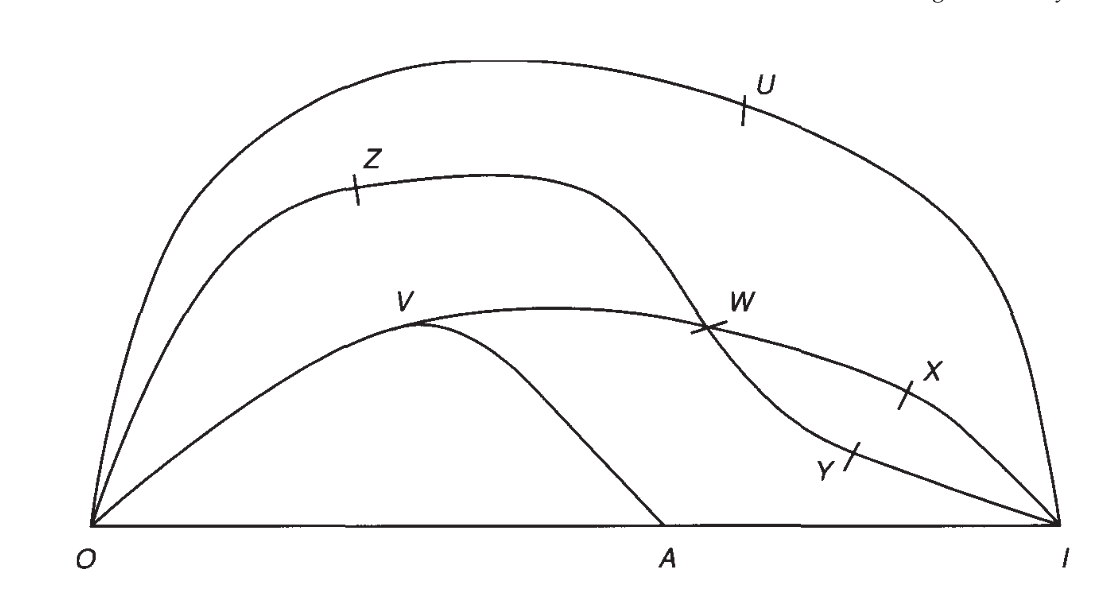
\includegraphics[scale=0.2]{./figures/Keynes.png}
		\end{figure}
\end{frame}



\begin{frame}
	\frametitle{Issues with Keynes' Theory}
	
	\begin{itemize}
		\item 	De Finetti regarded Keynes’s non-numerical probabilities as an \emph{unfortunate departure} from
		the \textbf{simplicity} and \textbf{power} of the mathematical theory of probability. He wrote:
		
		\begin{quote}
			Keynes’s position is certainly not suited to the development of a
			mathematical probability theory and is also hardly in keeping with the intuitive
			idea of probability.
			I myself regard as unacceptable, as a matter of principle, Keynes’s
			position (the more so since the reservations which he had disappear when
			one adopts a subjective point of view).
		\end{quote}
	\end{itemize}
\end{frame}

\begin{frame}
	\frametitle{Principle of Insufficient Reason}
	
	\begin{itemize}
		\item 	What then are the cases in which numerical values can be assigned to	probabilities? Keynes answers: 
		
		\begin{quote}
			‘In order that numerical measurement
			may be possible, we must be given a number of equally probable alternatives.’
		\end{quote}
		
		
		\item He even claims that this is something on which all probabilists agree:		
		
		\begin{quote}
			‘It has always been agreed that a numerical measure can actually be obtained in
			those cases only in which a reduction to a set of exclusive and exhaustive
			equiprobable alternatives is practicable.’
		\end{quote}
	\end{itemize}
\end{frame}

\begin{frame}
	\frametitle{Principle of Insufficient Reason}
	
	\begin{itemize}
		\item Keynes gives the following preliminary statement of the principle:
		

		\begin{quote}
			The Principle of Indifference asserts that if there is no known reason for
			predicating of our subject one rather than another of several alternatives,
			then relatively to such knowledge the assertions of each of these alternatives
			have an equal probability.
		\end{quote}		
	\end{itemize}
\end{frame}

\begin{frame}
	\frametitle{Logical Bayesianism}
	
	\begin{itemize}

		\item \textbf{Bayes Law}:
		\begin{equation*}
			\mathbb{P}(h|e) = \frac{\mathbb{P}(e|h) \mathbb{P}(h)}{\mathbb{P}(e)}
		\end{equation*}
		\pause
		\item If $e$ follows logically from $h$, then $\mathbb{P}(e | h) = 1$. If $h$ is a statistical hypothesis, an easy probability calculation often gives $\mathbb{P}(e | h)$.
		
		\pause
		\item Thus we need to evaluate $\mathbb{P}(h)$ and $\mathbb{P}(e)$; but how can this be done?
		
		\pause
		\item $h \in \{h_1, \dots, h_m\}$ and uniform!
		
		\pause
		\item $\mathbb{P} (e) = \sum_{i = 1}^{m} \underbrace{\mathbb{P}(h_i)}_{\frac{1}{m}} \mathbb{P}(e|h_i)$.
	\end{itemize}
\end{frame}

\begin{frame}
	\frametitle{On Principle of Insufficient Reason}
	\begin{itemize}
		\item This principle results in a lot of paradoxes!
		\pause
		
		\vspace{1cm}
		At the core of each paradox,  lies the following problem:
		\pause
		$$X \sim \mathrm{Unif}(0, 2) \text{    or    } X^2 \sim \mathrm{Unif} (0, 4)$$
	\end{itemize}
	
\end{frame}

\begin{frame}
	\frametitle{What comes next?}
	 In the next session, we will start discussing the \emph{Subjective Theory} of probability as a way to resolve issues we encountered when studying Logical probabilities.

\end{frame}


%\section{The Subjective Theory}
%\framecard{\LARGE The Subjective Theory}
%
%
%\section{The Frequency Theory}
%\framecard{\LARGE The Frequency Theory}
%
%
%\section{The Propensity Theory}
%\framecard{\LARGE The Propensity Theory}


\end{document}